% die Standard-Dokumentenklasse
\documentclass[11pt,a4paper]{article} %% 1.Ebene = chapter, headings

% input encoding, font encoding, outline font
\usepackage[utf8]{inputenc} 
\usepackage[T1]{fontenc} 
\usepackage{lmodern}
\usepackage{tcolorbox}
% Sprache
\usepackage[german]{babel}

% Absatzformatierung
\setlength{\parindent}{0pt}
\setlength{\parskip}{1ex plus 0.5ex minus 0.5ex}

% erweiterte mathematische Symbole
\usepackage{amsmath} 

% für Abbildungen
\usepackage{graphicx} 

% für Tabellen
\usepackage{booktabs}

% für Hyperlinks
\usepackage[colorlinks]{hyperref}
\graphicspath{}

%%%%%%%%%%%%%%%%%%%%%%%%%%%%%%%%%%%%%%%%%
\begin{document}


{
	\centering 
	\large 
	Physiklabor für Anfänger*innen \\
	Ferienpraktikum im Sommersemester 2018 \\[4mm]
	\textbf{\LARGE 
		Versuch 4: Dichte und Oberflächenspannung
	} \\[3mm]
	(durchgeführt am 07.09.2018 bei Daniel Bartle) \\
	Ye Joon Kim, Marouan Zouari\\
	\today \\[10mm]
}


\section{Einleitung}
Ein Wert auf mehrere Weisen zu messen ermöglicht es, die Genauigkeit der Messwerten zu verbessern und ein besseres Ergebnis. Zwei Methode, um die Dichte eines Objekts zu bestimmen, sind beispielsweise eine Jolly'sche Federwaage anzuwenden, oder direkt das Volumen und die Masse des jeweiligen Objekts zu messen. In dem ersten Versuchsteil werden beide Methode benutzt und verglichen. 

In dem 2. Versuchsteil wird die Oberflächenspannung, eine Quantifizierung der Kohäsion, von mehreren Flüssigkeiten bestimmt. 
\section{Ziel des Versuchs}
Das Ziel des ersten Teils des Versuchs ist es, die Dichte von festen Körpern und Flüssigkeiten zu bestimmen und beide Methodologien (beschrieben in Einleitung) zu vergleichen.

 Das Ziel des zweiten Teils ist es, die Oberflächenspannungen von Flüssigkeiten, nämlich von Wasser und Äthanol, zu bestimmen. 

\section{Aufbau}

\begin{figure}
	\centering
	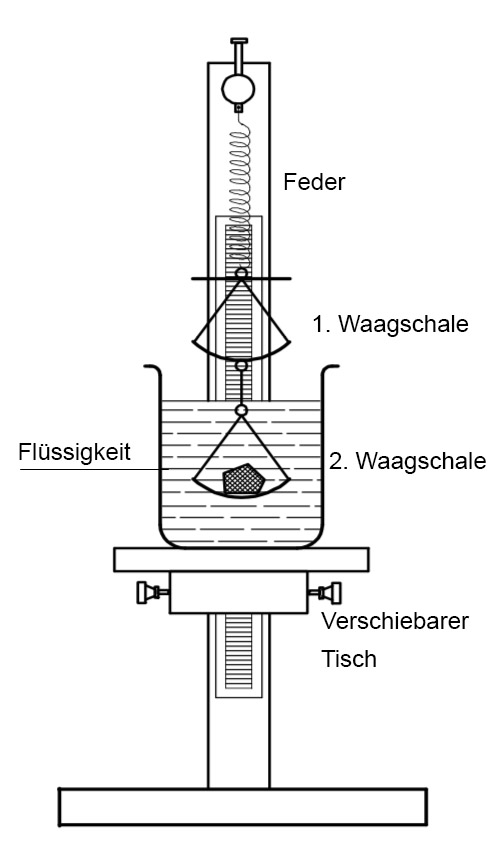
\includegraphics[scale=0.5]{Abb1}
	\caption { Jollysche Federwaage
		       (Aufbau zum 1. versuch) }
	               
	
	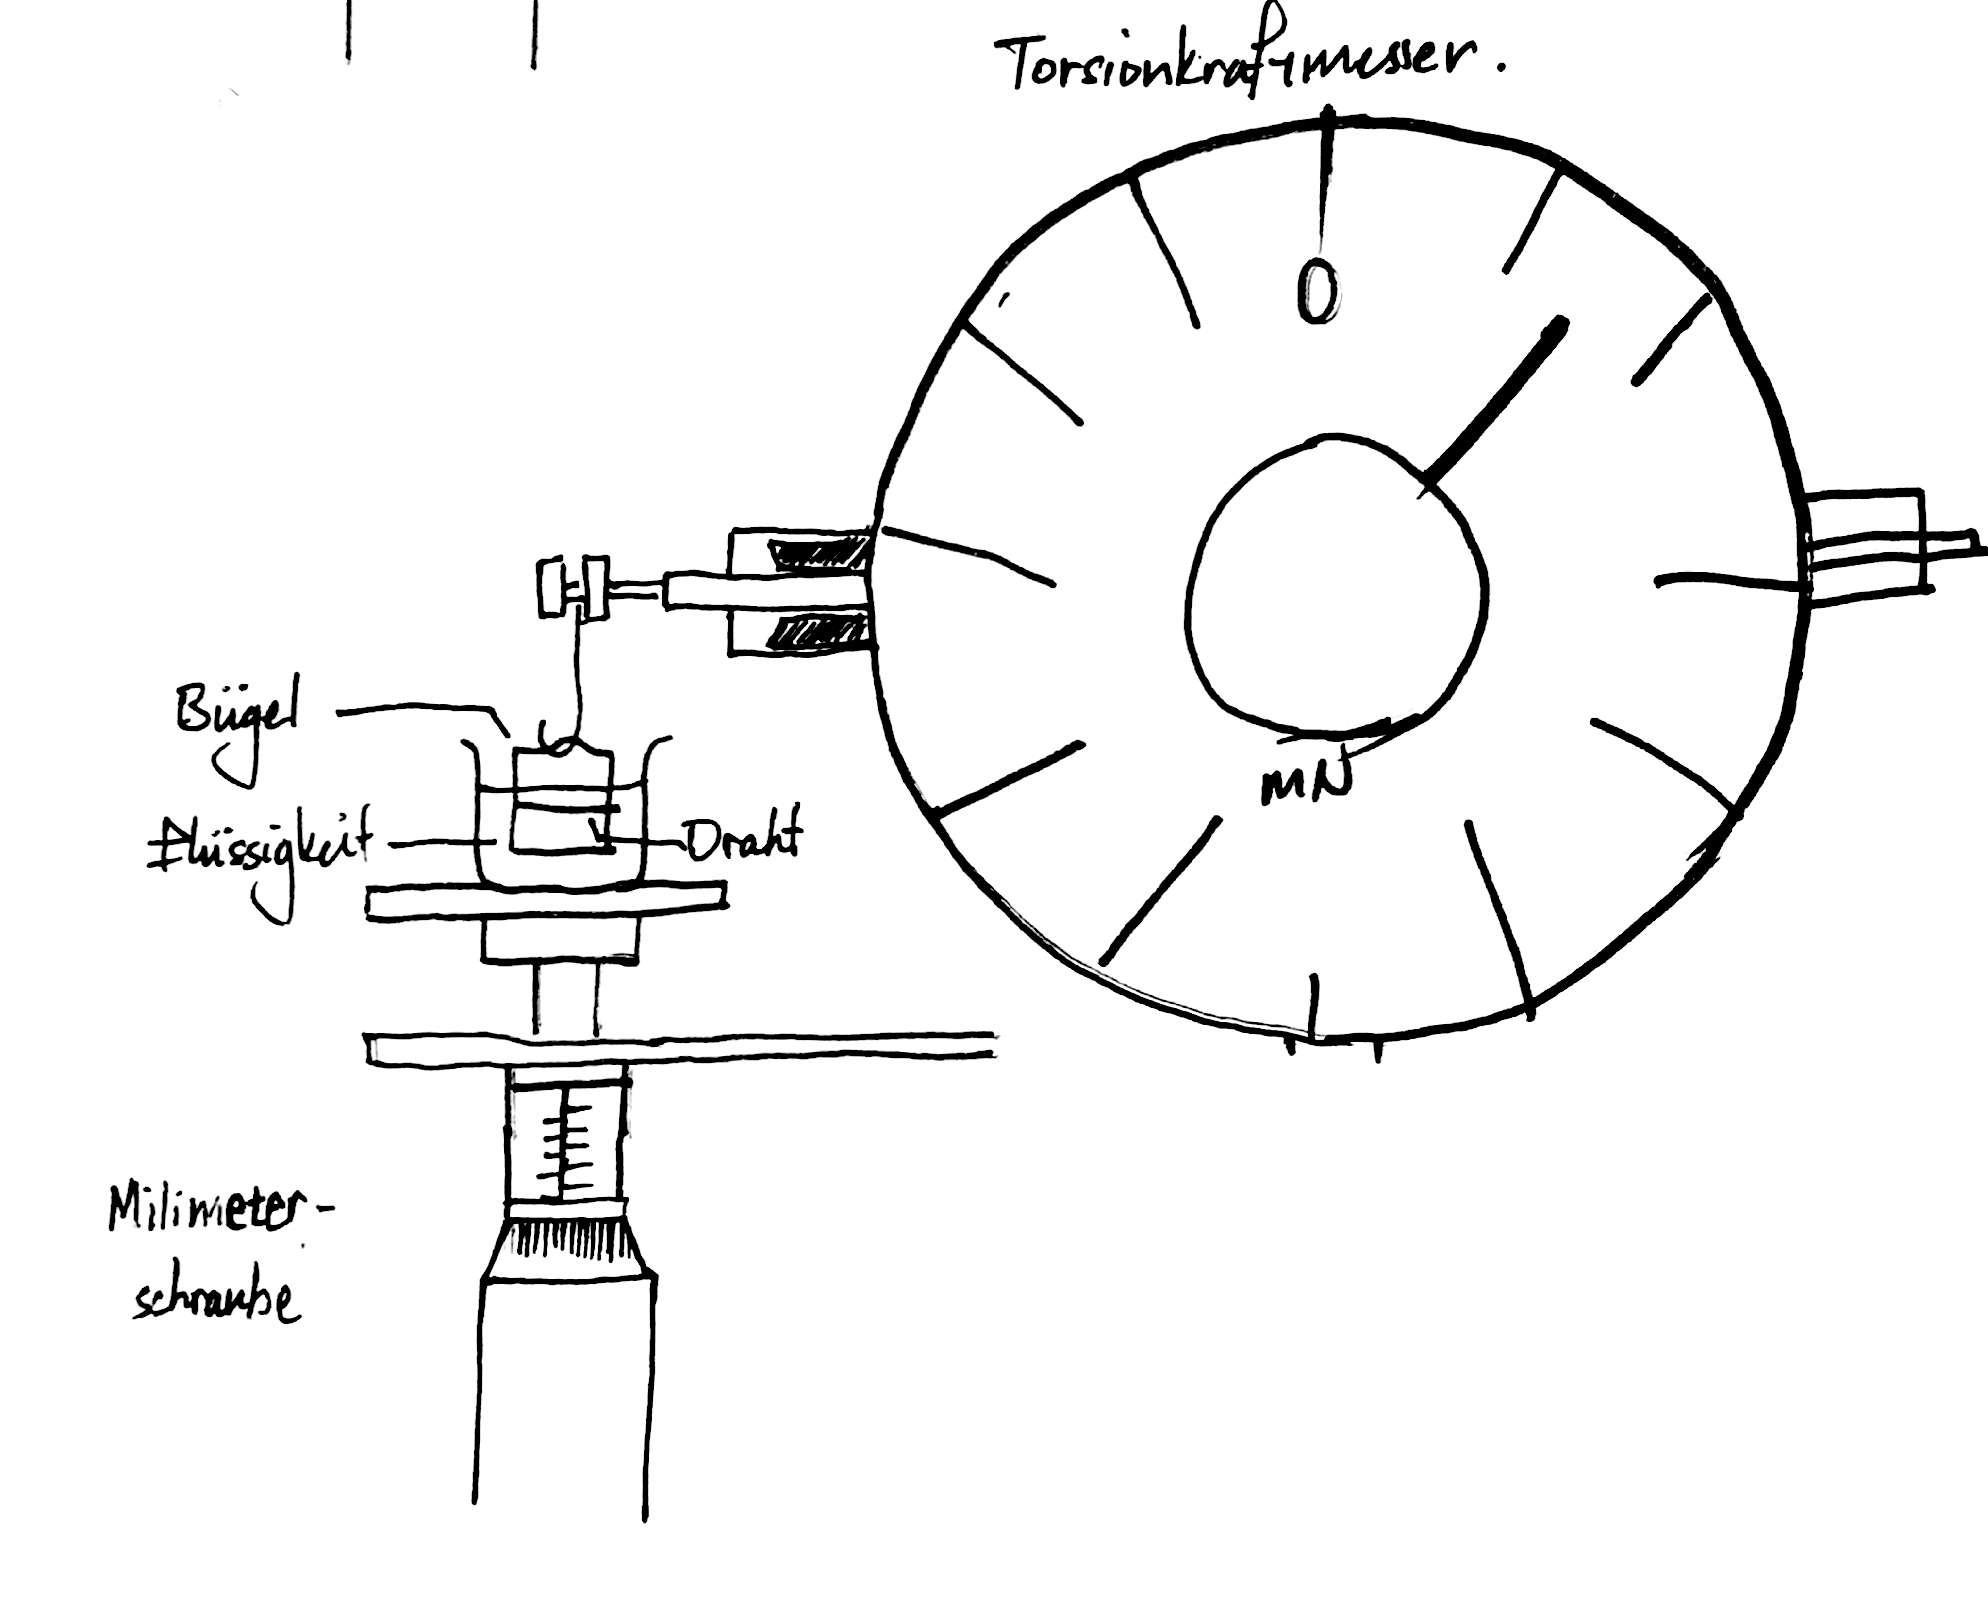
\includegraphics[scale=0.15]{Abb2}
	\caption{ Torsionskraftmessers 
		 (Aufbau zum 2. Versuchsteil)
	              }
\end{figure}
\newpage


\section{Auswertung und Fehleranalyse}

\subsection{1. Versuchsteil : Bestimmung der Dichte eines regulären Körpers:}
\subsubsection{Bestimung durch die Jolly'sche Fderwaage:}
Zur Bestimmung der Dichte wird die folgenden Formeln verwendet:

\begin{equation}
\frac{\rho}{\rho_{Fl}} = \frac{F_{G}}{F_{A}} = \frac{F_G}{F_G - F_{G'}}
\end{equation}

\begin{equation}
F = -k\cdot(x-x_0)
\end{equation}

Wobei für (1):
\begin{itemize}
	\item $\rho$ und $\rho_{Fl}$ die Dichten des Körpers und bzw. der Flüssigkeit 
	\item $F_G$ die auf den Körper wirkende Gravitationskraft
	\item $F_{G'}$ die auf den in der Flüssigkeit eingetauchten Körper wirkende Gravitationskraft
	\item $F_A$ die Auftriebskraft
\end{itemize}

und für (2):
\begin{itemize}
	\item $F$ die Federkraft
	\item $k$ die Federkonstante
	\item $x_0$ die Ruhelage des Fadens und Schale
\end{itemize}

Das Einsetzen von Gleichung (2) in Gleichung (1) liefert: 
\begin{equation}
\frac{\rho}{\rho_{Fl}} = \frac{x_1-x_0}{(x_1-x_0)-(x_2-x_0)}
\end{equation}

Für die Erleichterung der Berechnung wurden zuerst die Differenzen, die in der obigen Formel auftauchen, und deren Unsicherheiten berechnet

\begin{table}[h]
	\begin{tabular*}{0.99\textwidth}{@{\extracolsep{\fill}}cccccc}
		\toprule
		$x_1-x_0$ & $\Delta (x_1-x_0)$ &  $x_2-x_0$  &  $\Delta(x_2-x_0)$  \\
		mm & mm &  mm & mm   \\
		\midrule
		17 & 1 & 3 & 1 \\
		19 & 1 & 3 & 1 \\
		20 & 1 & 2 & 1 \\
		18 & 1 & 2 & 1 \\
		
		\bottomrule
	\end{tabular*}
	\caption{Die Differenzen zwischen $x_1$ und $x_0$ und zwischen $x_2$ und $x_1$ sowie deren Unsicherheiten}
	\label{tabelle}
\end{table}



\begin{tcolorbox}[colback=white]
\textbf{Beispilerechnung:}
      Siehe Anhang: Rohe Daten Tabella 8
$$x_1-x_0=$$
$$395\textrm{mm}-412\textrm{mm}=$$
$$17\textrm{mm}$$

Für die Unsicherheiten der Differenzen wurden die Gauß'sche Fehlerfortpflanzung benutzt.

Sei:
$$f(x_1,x_0)=x_1-x_0$$
$$\frac{\partial f}{\partial x_0}=1$$
$$\frac{\partial f}{\partial x_1}=1$$
Dann ist:
$$\Delta({x_1-x_0})=\sqrt{(\frac{\partial f}{\partial x_0}\Delta{x_0})^2+(\frac{\partial f}{\partial x_1}\Delta{x_1})^2}$$
$$=\sqrt{1\cdot(1\textrm{mm})^2+1\cdot(1\textrm{mm})^2}$$
$$=\sqrt{2}\textrm{mm}\approx1,414\textrm{mm}$$
Das wird gerundet zu:
$$\Delta{x_1-x_0}=1\textrm{mm}$$
\end{tcolorbox}
\hrule

\vspace{5mm}
Danach werden die Mittelwerte der Differenzen sowie deren Unsicherheiten berechnet. 

\begin{table}[h]
	\begin{tabular*}{0.99\textwidth}{@{\extracolsep{\fill}}cccccc}
		\toprule
		$\overline{x_1-x_0}$ & $u_{\overline{x_1-x_0}}$ &  $\overline{x_2-x_0}$  &  $u_{\overline{x_2-x_0}}$  \\
		mm & mm &  mm & mm   \\
		\midrule
		19 & 1 & 3 & 1 \\
		
		\bottomrule
	\end{tabular*}
	\caption{Die Mittelwerte der Differenzen und ihre Unsicherheiten}
	\label{tabelle2}
\end{table}


\begin{tcolorbox}[colback=white]
	\textbf{Beispilerechnung:}
$$\bar{x}=\frac{\sum x}{n}$$
$$\overline{x_1-x_0}=\frac{17\textrm{mm}+19\textrm{mm}+20\textrm{mm}+18\textrm{mm}}{4}$$
$$=18,5\textrm{mm}$$

und für die Unsicherheiten werden die Standardunsicherheiten benutzt:
\begin{equation}
u_{x}=\sqrt{\frac{\sum(x-\bar{x})^2}{n-1}}
\end{equation}
$$u_{\overline{x_1-x_0}}=\sqrt{\frac{(1,5\textrm{mm})^2+(0,5\textrm{mm})^2+(1,5\textrm{mm})^2+(0,5\textrm{mm})^2}{3}}$$
$$\approx1,29\textrm{mm}\approx1\textrm{mm}$$
\end{tcolorbox}
\vspace{5mm}

Eingesetzt in Formel (3) ergibt:
$$\frac{\rho}{\rho_{Fl}} = 1.16 \pm0,07$$


\begin{tcolorbox}[colback=white]
	\textbf{Beispilerechnung:}
$$\frac{\rho}{\rho_{Fl}} = \frac{x_1-x_0}{(x_1-x_0)-(x_2-x_0)}$$
$$=\frac{18,5\textrm{mm}}{18,5\textrm{mm}-2,5\textrm{mm}}$$
$$\approx1,16$$
Für die Fehler dieses Verhältnisses wird erneut die Gaußsche Fehlerfortpflanzung benutzt.Mit:
$$f((x_1-x_0),(x_2-x_0))=\frac{x_1-x_0}{(x_1-x_0)-(x_2-x_0)}$$
sind
$$\frac{\partial f}{\partial (x_1-x_0)}=-\dfrac{x_2-x_0}{\left((x_1-x_0)-(x_2-x_0)\right)^2}$$
$$\frac{\partial f}{\partial (x_2-x_0)}=\dfrac{x_1-x_0}{\left((x_2-x_0)-(x_1-x_0)\right)^2}$$
und mit
$$\Delta{\frac{\rho}{\rho_{Fl}}}=\sqrt{(\frac{\partial f}{\partial (x_1-x_0)}u_{\overline{x_1-x_0}})^2+(\frac{\partial f}{\partial (x_2-x_0)}u_{\overline{x_2-x_0}})^2}$$
ist die Unsicherheit
$$\approx0,0724\approx0,07$$
\end{tcolorbox}
\hrule
\vspace{5mm}

Die Dichte von Wasser bei $25^\circ$C ist 997.05 kg/m$^3$.

Die Dichte des Körpers ist deshalb:
$$\rho=(1160\pm70) \textrm{kg/m}^3$$

Die Unsicherheit der Dichte lässt sich auch mit der Standardabweichung der von den einzelnen Messreihen gewonnenen Dichten bestimmen.
Mit Gleichung (4) ist die Standardunsicherheit der Dichten:
$$u_\rho=49,24{kg/m}^3$$



\subsubsection{Bestimmung durch Volumen und Masse}
Die Dichte eines Objekts lässt sich auch mit die folgende Formel bestimmen. 
\begin{equation}
\rho=\frac{m}{V}
\end{equation}
Wobei $m$ und $V$ die Masse bzw. Volumen des Objekts sind. 

Die Volumen des Objekts $V$ ist:
$$(4,7\pm0,2) \textrm{cm}^3 = (0,0047 \pm 0,0002) \textrm{m}^3$$
und der Masse $m=(5,55\pm0,01)\textrm{g}$ ist die Dichte:
$$(1170 \pm 50) \textrm{kg/m}^3$$

\begin{tcolorbox}[colback=white]
	\textbf{Beispilerechnung:}
	
Für das Volumen benutzen wir die folgende Formel:
$$V = \pi (\frac{d}{2})^2 h$$
Wobei d und h der Durchmesser bzw. die Höhe des Zylinders sind. 
$$V = \pi (\frac{1,6\textrm{cm}}{2})^2\cdot2,35\textrm{cm}$$
$$ = 4,725 \textrm{cm}^3$$
Dadurch ist die Dichte:
$$\rho=\frac{5,55\textrm{g}}{4,725\textrm{cm}^3}$$
$$=1,1746\textrm{g/cm}^3=1174,6\textrm{kg/m}^3$$

Zur Fehlerrechnung wird die Gaußsche Fehlerfortpflanzung benutzt. Mit $f(d,h)=\pi(\frac{d}{2})^2h$ 
$$u_V = 0,2390 \textrm{cm}^3$$
 (Verfahren wie in 3.1.3).

 Die Unsicherheit der Dichte lässt sich mit der vereinfachte Formel für Produkte und Quotienten bestimmen. 
\begin{equation}
\vert\frac{\Delta z}{z_0}\vert = \sqrt{(a\frac{\Delta x}{x_0})^2+(b\frac{\Delta y}{y_0})^2} \; \; \textrm{für} z=x^a\cdot y^b
\end{equation}
$$|\frac{\Delta\rho}{\rho}|=\sqrt{(1\cdot\frac{0,01\textrm{g}}{5,55\textrm{g}})^2+(-1\cdot\frac{0,2\textrm{cm}^3}{4,7\textrm{cm}^3})^2}$$
$$=0,426$$
Daraus folgt:
$$\Delta\rho=50,00\textrm{kg/m}^3$$
\end{tcolorbox}

\newpage
\subsection{2. Teil: Bestimmung der Dichte einer unbekannten Flüssigkeit}

\begin{table}[ht]
	\begin{tabular*}{0.99\textwidth}{@{\extracolsep{\fill}}cccccc}
		\toprule
		$x_1-x_0$ & $\Delta(x_1-x_0)$ &  $x_2-x_0$  &  $\Delta(x_2-x_0)$  \\
		mm & mm &  mm & mm   \\
		\midrule
		20 & 1 & 7 & 1 \\
		19 & 1 & 7 & 1 \\
		19 & 1 & 7 & 1 \\
		19 & 1 & 6 & 1 \\
		
		\bottomrule
	\end{tabular*}
	\caption{Die Differenzen zwischen $x_1$ und $x_0$ und zwischen $x_2$ und $x_1$ sowie deren Unsicherheiten}
	\label{tabelle3}
\end{table}

Die Mittelwerte und deren Unsicherheiten lauten:


\begin{table}[ht]
	\begin{tabular*}{0.99\textwidth}{@{\extracolsep{\fill}}cccccc}
		\toprule
		$\overline{x_1-x_0}$ & $u_{\overline{x_1-x_0}}$ &  $\overline{x_2-x_0}$  &  $u_{\overline{x_2-x_0}}$  \\
		mm & mm &  mm & mm   \\
		\midrule
		19 & 1 & 7 & 1 \\
		
		\bottomrule
	\end{tabular*}
	\caption{Die Mittelwerte der Differenzen und ihre Unsicherheiten}
	\label{tabelle4}
\end{table}

Die Werte Eingesetzt in Formel (3) liefert:
$$\frac{\rho}{\rho_{Fl}}=1,54\pm0,10$$

Die Berechnungsverfahren sind genau wie in dem 1. Teil. 

Die Umformung der obigen Formel liefert:
$$\rho_{Fl}=\frac{\rho}{1,54\pm0,10}$$
Und von Teil 1 wissen wir dass $\rho=(1160\pm70) \textrm{kg/m}^3$. $\rho_{Fl}$, die Dichte der unbekannten Flüssigkeit ist deshalb:
$$\rho_{Fl}=750 \pm 70 \textrm{kg/m}^3$$
und die Standardabweichung (Standardunsicherheit) der einzelnen Dichtmessungen ist:
$$u_{\rho_{Fl}}=28,78\textrm{kg/m}^3\approx30\textrm{kg/m}^3$$

\begin{tcolorbox}[colback=white]
	\textbf{Beispilerechnung:}
$$\rho_{Fl}=\frac{\rho}{1,54}$$
$$=\frac{1160 \textrm{kg/m}^3 }{1,54}$$
$$=753,24 \textrm{kg/m}^3\approx 750 \textrm{kg/m}^3$$

für die Unsicherheit wird die vereinfachte Formel für Produkte und Quotienten benutzt.(Formel (5))


$$\vert\frac{\Delta{\rho_{Fl}}}{\rho_{Fl}}\vert = \sqrt{(\frac{1,54}{0,10})^2+(\frac{1160 \textrm{kg/m}^3}{70\textrm{kg/m}^3})^2}$$

$$\frac{u_{\rho_{Fl}}}{\rho_{Fl}} = 0,0886$$
$$u_{\rho_{Fl}}={\rho_{Fl}}\cdot0,0886=753,24\textrm{kg/m}^3\cdot0,0886$$
$$\approx66,74\textrm{kg/m}^3\approx70\textrm{kg/m}^3$$
\end{tcolorbox}


In dem 2. Teil ist auch ein Systematischer Fehler zu berücksichtigen. Aufgrund der Unsicherheit der Dichtmessung in dem 1. Versuchsteil können die berechneten Werten zu hoch oder zu klein abgeschätzt werden sein. 

\subsection{2. Versuchsteil: Bestimmung der Oberflächenspannung}
\newpage
\begin{figure}[h!]
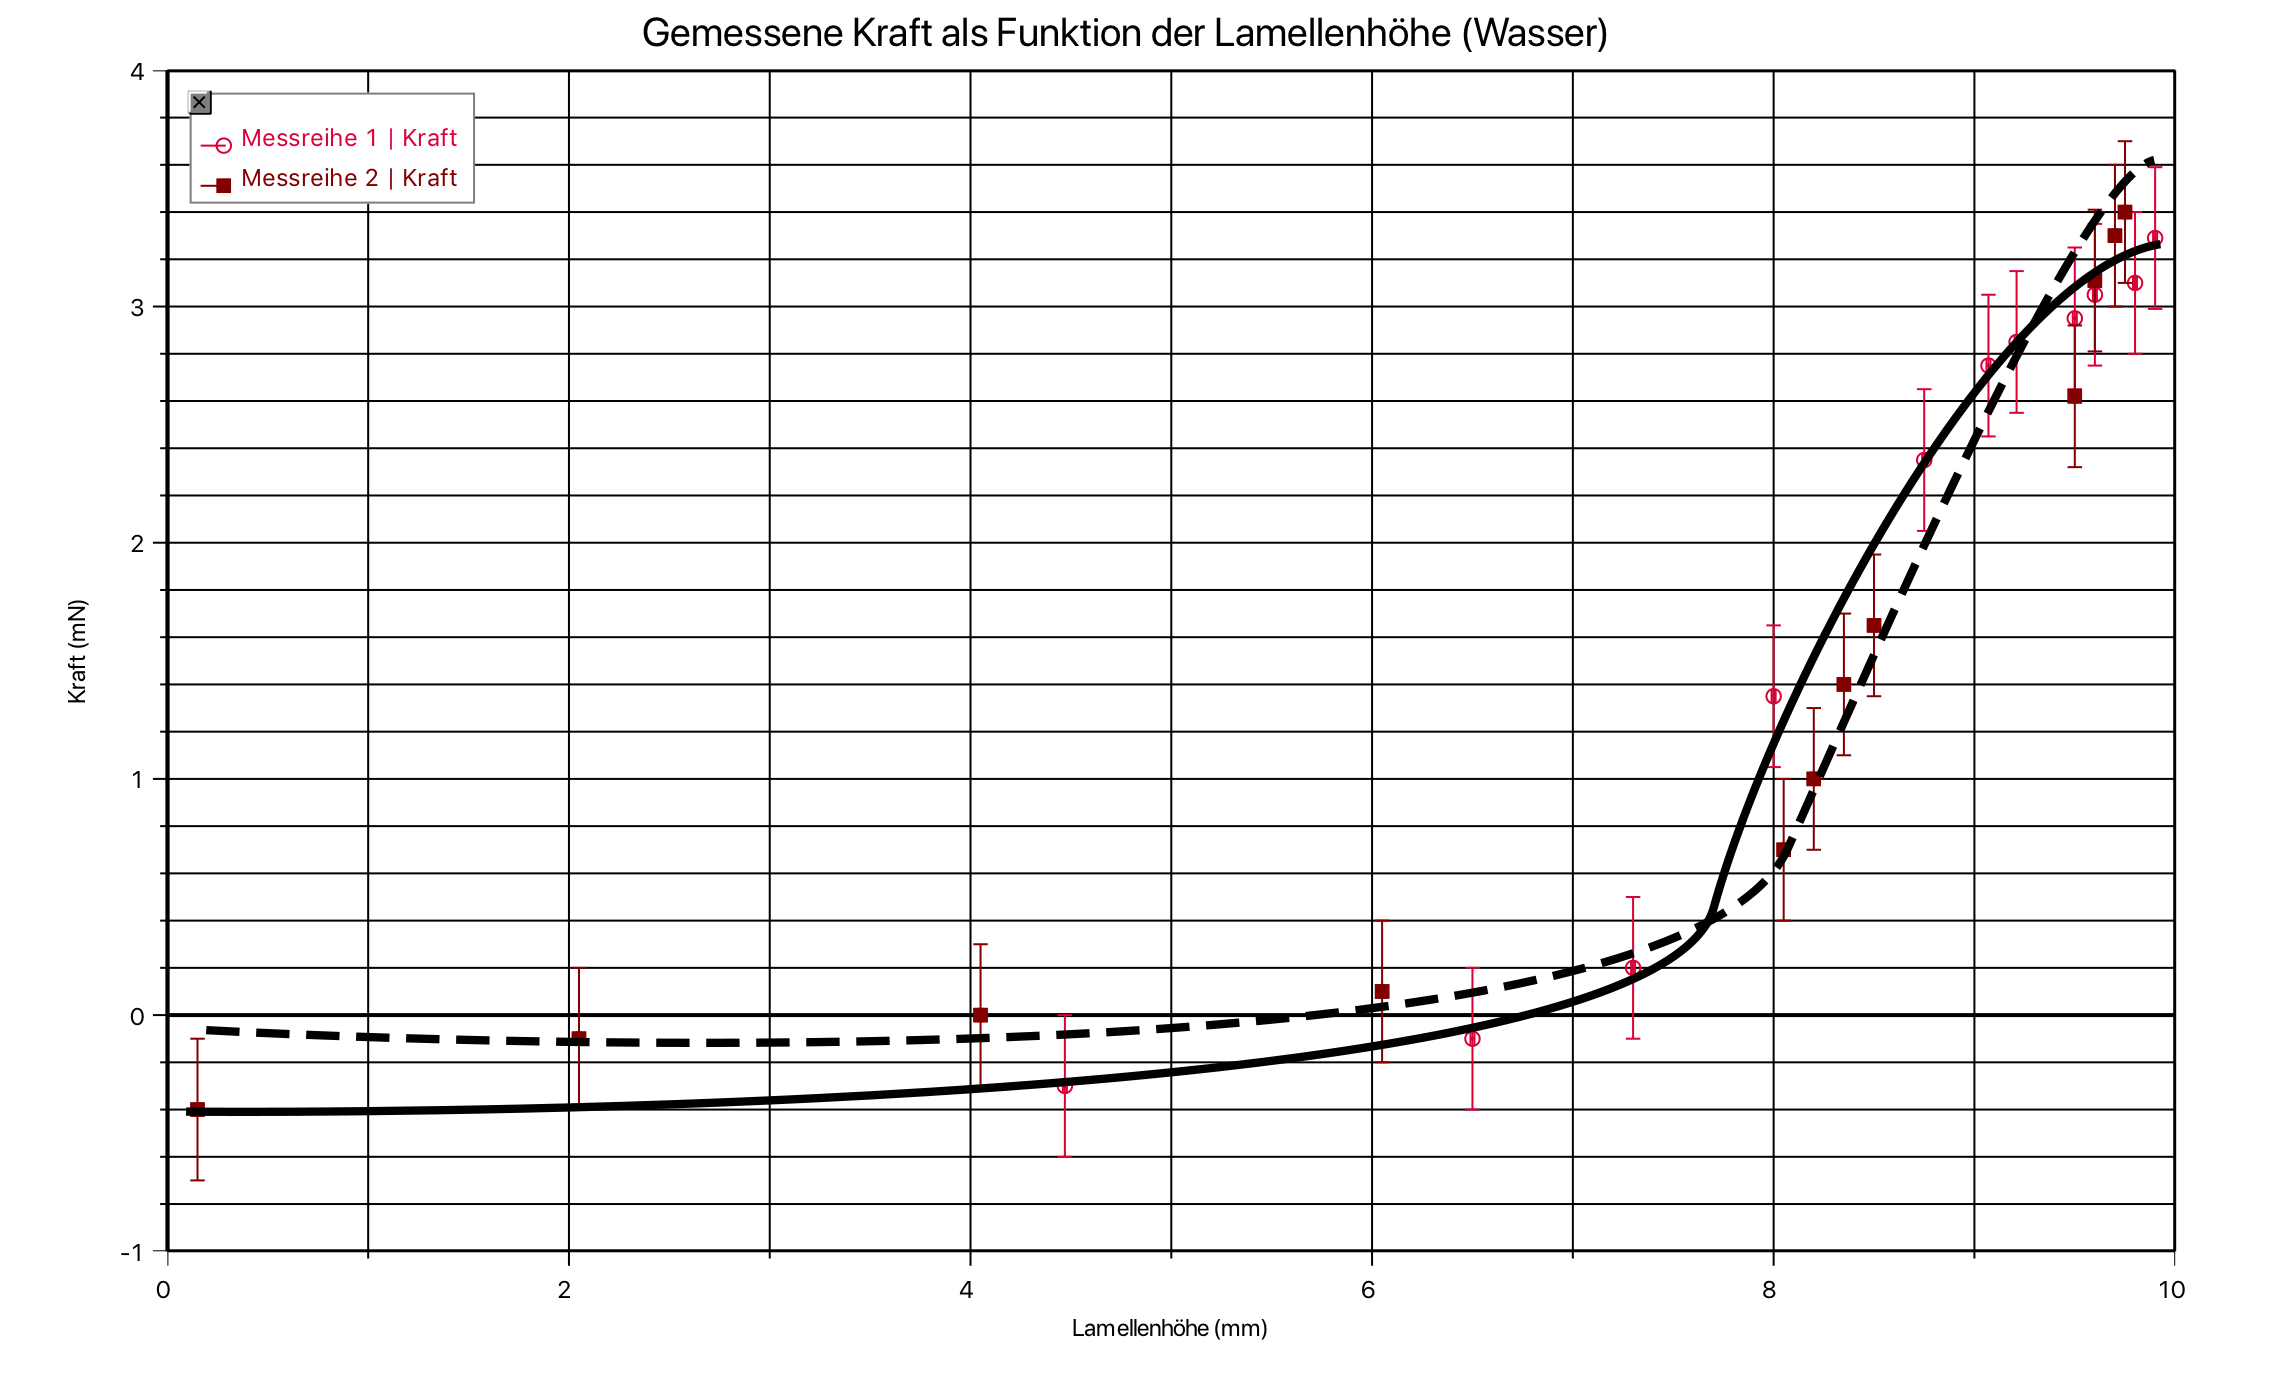
\includegraphics[width=\textwidth]{ex4gr1}
\caption{Verlauf der Kraft $F$ als Funktion der Lamellenhöhe sowie dessen Fit-Kurven bei Wasser.(Gepunktete Linie für die 2. Messreihe)}

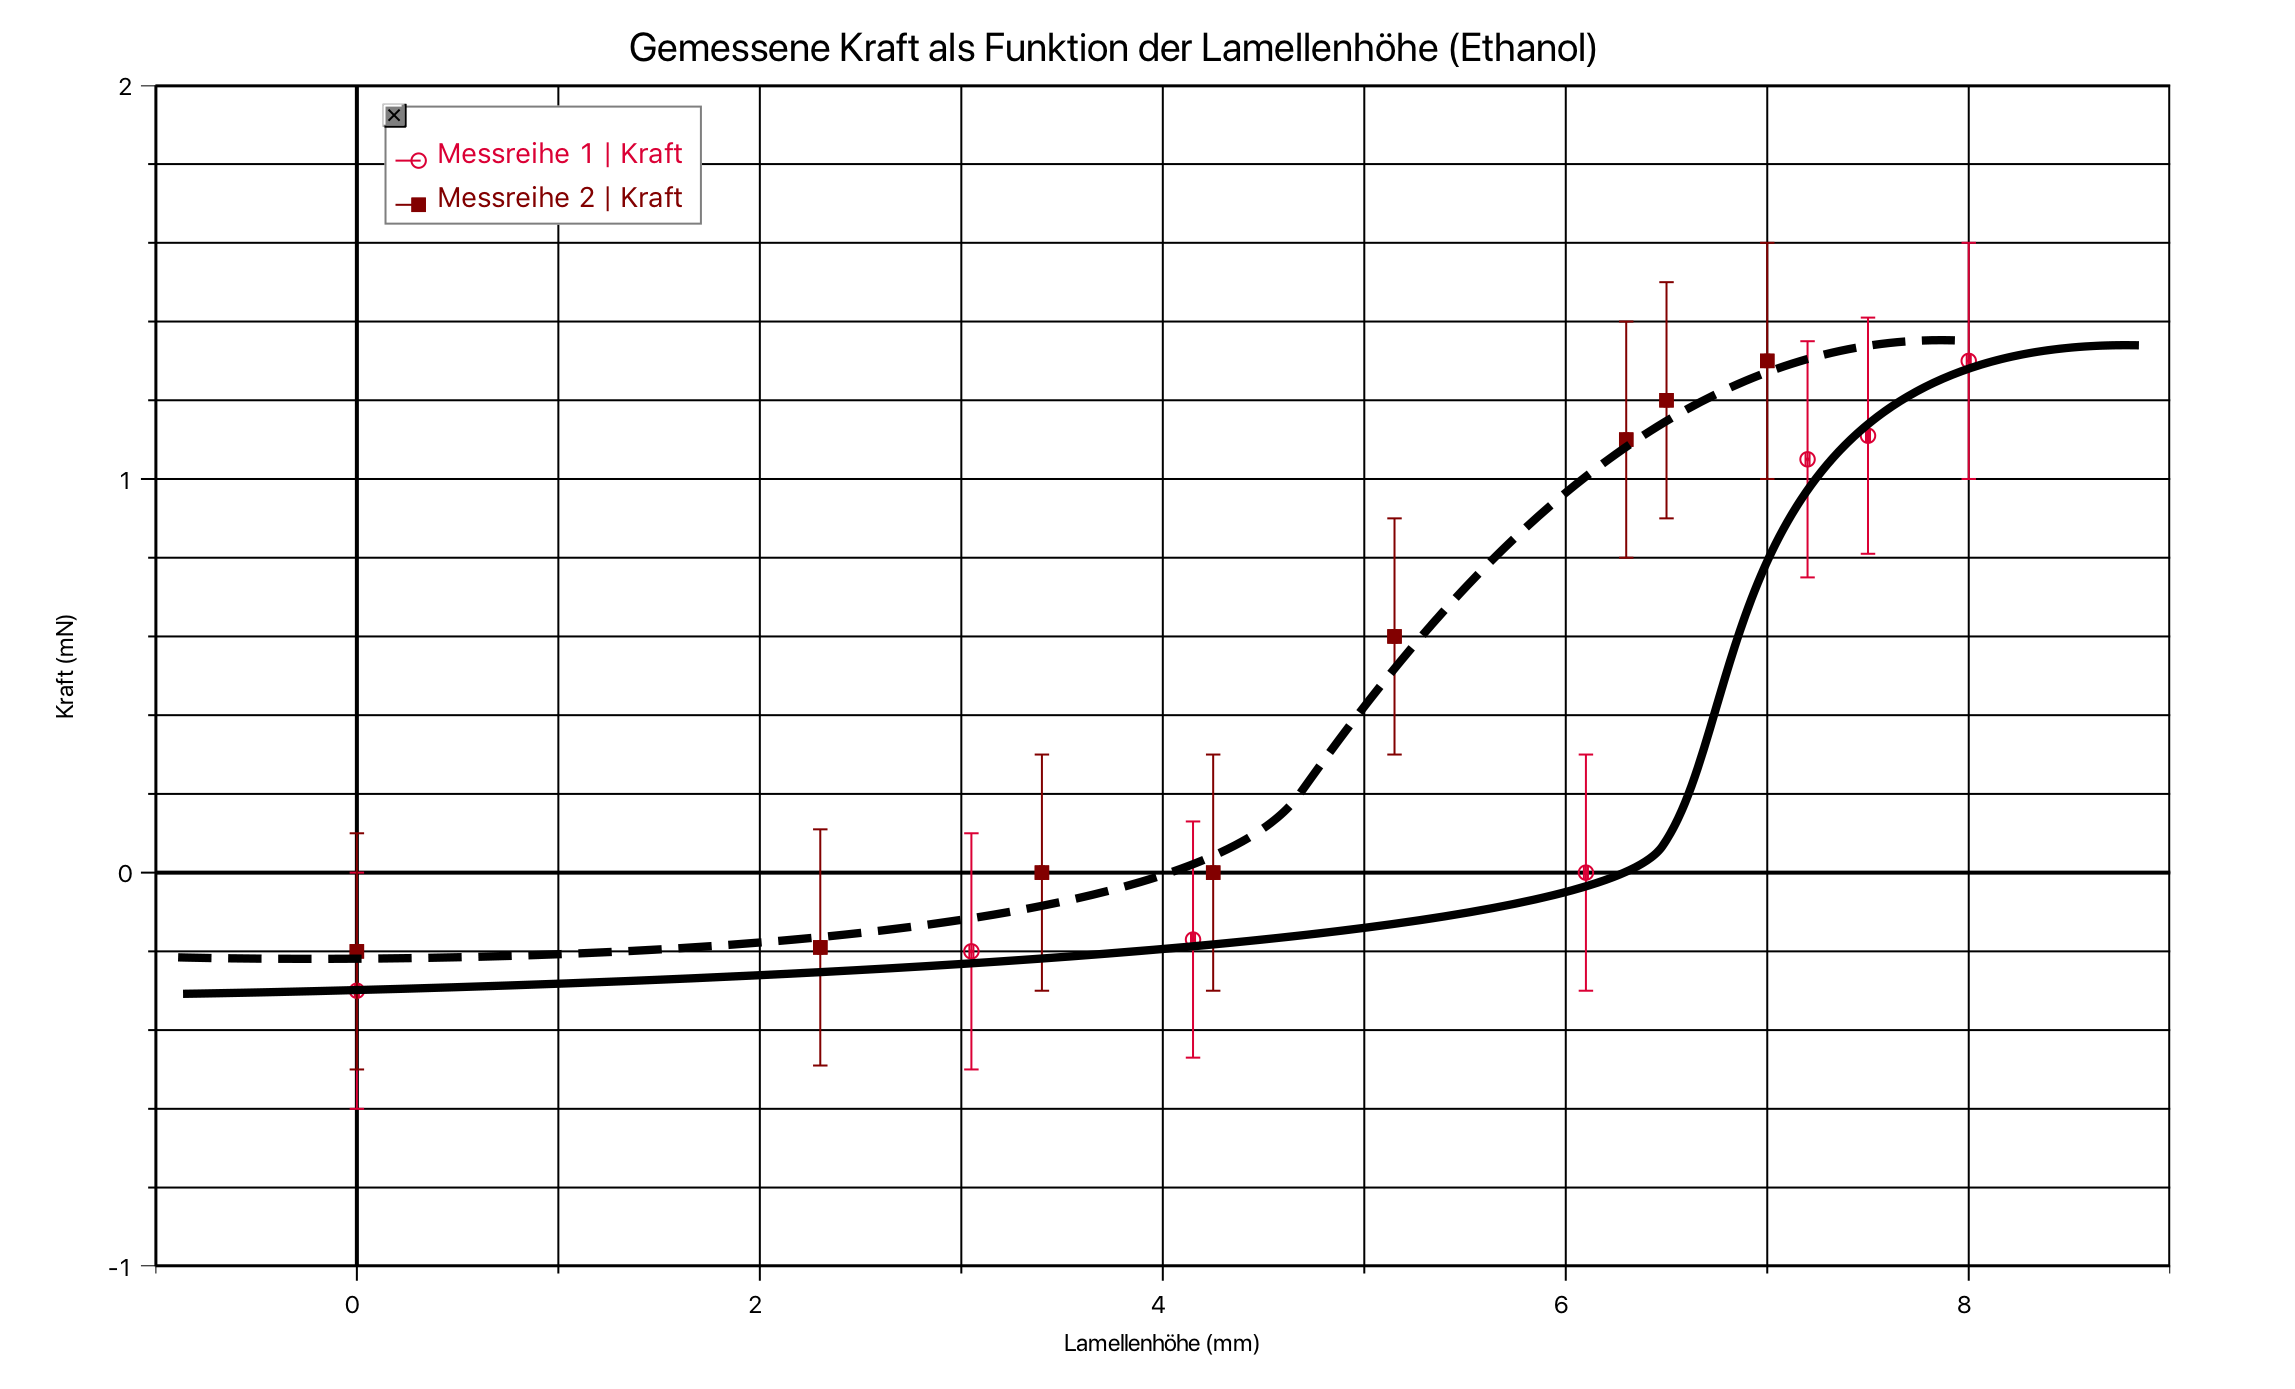
\includegraphics[width=\textwidth]{ex4gr2}
\caption{Verlauf der Kraft $F$ als Funktion der Lamellenhöhe sowie dessen Fit-Kurven bei Ethanol.(Gepunktete Linie für die 2. Messreihe)}
\end{figure}
\newpage

Die gemessene Länge des Messdrahtes war:
$$l=2,530 \pm 0,005 \textrm{cm}$$


Die einzelne $F(s_{\textrm{max}})$ wurden direkt von den Diagrammen mit dem Fit-Kurven abgelesen, und deren Unsicherheiten als 0,3 \textrm{mN} genommen. Dadurch lassen sich die jeweilige Oberflächenspannungen bestimmen. 


\begin{table}[h]
	\begin{tabular*}{0.99\textwidth}{@{\extracolsep{\fill}}cccccc}
		\toprule
		$F(s_{\textrm{max}})$ & $\Delta{F(s_{\textrm{max}})}$ & $\sigma$ & $\Delta\sigma$  \\
		mN & mN &  mN/cm & mN/cm   \\
		\midrule
		3,3 & 0,3 &  1,3 & 0,1 \\
		3,4 & 0,3 & 1,3 & 0,1 \\
		
		\bottomrule
	\end{tabular*}
	\caption{Kraft $F(s_\textrm{max})$ bei der maximalen Lamellenhöhe und die entsprechenden Oberflächenspannungen in Wasser}
	\label{tabelle5}
\end{table}

\begin{table}[h]
	\begin{tabular*}{0.99\textwidth}{@{\extracolsep{\fill}}cccccc}
		\toprule
		$F(s_{\textrm{max}})$ & $\Delta{F(s_{\textrm{max}})}$ & $\sigma$ & $\Delta\sigma$  \\
		mN & mN &  mN/cm & mN/cm   \\
		\midrule
		1,3 & 0,3 & 0,27  & 0,06 \\
		1,3 & 0,3 & 0,27 & 0,06 \\
		
		\bottomrule
	\end{tabular*}
	\caption{Kraft $F(s_\textrm{max})$ bei der maximalen Lamellenhöhe und die entsprechenden Oberflächenspannungen in Ethanol}
	\label{tabelle6}
\end{table}
 
Für die Berechnung der Unsicherheiten wird die vereinfachte Formel für Produkte und Quotienten benutzt. Das Berechnungsverfahren ist genau wie in dem 1. Teil dargestellt. 
Die Mittelwerte und ihre Unsicherheiten lauten:


\begin{table}[h]
	\begin{tabular*}{0.99\textwidth}{@{\extracolsep{\fill}}cccccc}
		\toprule
		$\overline{\sigma}_{\textrm{Wasser}}$ & $u_{\overline{\sigma}\textrm{Wasser}}$ & $\overline{\sigma}_{\textrm{Ethanol}}$ & $\Delta\overline{\sigma}_{\textrm{Ethanol}}*$  \\
		mN & mN &  mN/cm & mN/cm   \\
		\midrule
		1,32 & 0,03 & 0,26  & 0,04 \\
		
		\bottomrule
	\end{tabular*}
	\caption{Die Mittelwerte der berechneten Oberflächenspannungen in Wasser und Ethanol und ihre Unsicherheiten.}
	\label{tabelle7}
\end{table}
*Da die gemessene Oberflächenspannungen für beide Messreihen dieselben Werte hatten, wurde die statistische Unsicherheit der Einzelmessung mit einer Skalierung für Mehrfachmessungen (nämlich $\frac{1}{\sqrt{2}}$) benutzt.

\section{Diskussion der Ergebnisse}
\subsection{1. Versuchsteil}
Die mit der Jolly'schen Federwaage gemessenen Dichte des Zylinders ist:
$$(1160\pm 70)\textrm{kg/m}^3$$
und die durch Gewicht- und Volumenmessungen bestimmten Dichte:
$$(1170\pm 50)\textrm{kg/m}^3$$
Da beide Werte innerhalb ihrer Unsicherheiten liegen, stimmen beide Werte überein. 

Die berechnete Dichte der unbekannten Flüssigkeit ist:
$$(750 \pm 70) \textrm{kg/m}^3$$

Ein möglicher Systematischer Fehler könnte sein, dass die Messungen mit einem nicht idealen Feder durchgeführt wurden. Deshalb könnte es Abweichungen von der linearen Beziehung zwischen Kraft und Abstand geben. In diesem Fall sind die benutzten Formeln von schlechten Modellen und liefern falsche Ergebnisse. 
die sch\"{u}tzung der Feder von aussern Factoren wie grosse 
Temperaturwechsel, Luft Feuchtigkeit und extreme mechanische kr\"{a}fte sind m\"{o}glicher l\"{o}sungen. Auch ist die Herstellung der Feder aus widerstandsfähigem Materialen , die diese Faktoren nicht leicht beeinträchtigt.

Eine statistische Unsicherheit ist die Dicke der horizontalen Komponente der Waage, mit der die Höhe der Schalen abgelesen werden kann. Die Dicke könnte zu einer Ungenauigkeit von dem Ablesen von den Auslenkungen $x_0$, $x_1$ usw. auf der Skala führen. Dieses Problem lässt sich dadurch lösen, indem man diese Komponente dünner macht. 

\subsection{2. Versuchsteil}
Es wurde berechnet, dass die Oberflächenspannung von Wasser ist:
$$(1,32\pm 0,03) \textrm{mN/cm}$$
und die von Ethanol:
$$(0,257 \pm 0,04) \textrm{mN/cm}$$

Eine große Systematische Unsicherheit war es, dass  $F(s_\textrm{max})$ nicht direkt bestimmt werden konnte. Die letzten Messwerte sind die Werte, die gemessen wurden, bevor die Lamelle gerissen war. Das heißt, die letzten Datenpunkte liegen alle unter dem wirklichen $F(s_\text{max})$. 

Zusätzlich ist ein statistischer Fehler, dass die Werte für $F(s_\textrm{max})$ von einer selbst gezeichneten Kurve abgeschätzt werden mussten. Es können mehrere Kurven geben, die mit den Datenmessungen passen, und je nach dem, wie man die Kurven zeichnen, können die abgelesenen Werte für $F(s_\textrm{max})$ anders sein. 

Beide Probleme lassen sich dadurch verbessern, indem man die Mikrometerschraube langsamer dreht und Messungen häufiger macht. 

\newpage
\section{Anhang: Rohe Daten}
\subsection{1. Versuchsteil}
\begin{table}[h]
	\begin{tabular*}{0.99\textwidth}{@{\extracolsep{\fill}}cccccc}
		\toprule
		$x_1$ & $x_2$ &  $x_0$    \\
		mm & mm &  mm    \\
		\midrule
		395 & 409 & 412 \\
		441 & 457 &  460 \\
		412 &  430 & 432  \\
		402 & 418 & 420 \\
		
		\bottomrule
	\end{tabular*}
	\caption{Gemessene Werte für $x_1$, $x_2$ und $x_0$ (1. Teil)}
	\label{tabelle}
\end{table}
\begin{table}[h]
	\begin{tabular*}{0.99\textwidth}{@{\extracolsep{\fill}}cccccc}
		\toprule
		$x_1$ & $x_2$ &  $x_0$    \\
		mm & mm &  mm    \\
		\midrule
		391 & 404 & 411 \\
		384 & 396 &  403 \\
		413 &  425 & 432  \\
		440 & 453 & 459 \\
		
		\bottomrule
	\end{tabular*}
	\caption{Gemessene Werte für $x_1$, $x_2$ und $x_0$ (2. Teil)}
	\label{tabelle}
\end{table}

\subsection{2. Versuchsteil}
Da die Tabellen zu lang sind, bitte siehe Zusatzblätter für die rohen Daten zum 2. Versuchsteil. 


%lots of problems with the Jollysche Federwaage. Statis:The Feder may not be 
%System: The Kraft may not be linear. The condition of the spring may affect its performance. (Such as geometrical deformation from perfect circle). Einfluss der Federkonstante (nichtidealer Feder) nach Länge. Formula may not reflect real force.


\newpage
\section{Literatur}
"Dichte."\space Wikipedia

"Versuchseinleitungen zum Physiklabor für Anfänger*innen, Teil 1." \space  Albert-Ludwigs-Universität Freiburg, 2018. 



\end{document}